% Compile with XeLaTeX twice, or: tectonic report.tex
\documentclass[UTF8,fontset=fandol,a4paper,10pt]{ctexart}
\usepackage[margin=18mm,top=15mm,bottom=16mm]{geometry}
\usepackage{graphicx,booktabs,array,xcolor,tikz,caption,hyperref,amsmath}
\usetikzlibrary{arrows.meta,positioning}
\hypersetup{colorlinks=true,urlcolor=blue!55!black,pdftitle={ACPV-Net在IRSAMap上的微调简报}}
\definecolor{ink}{HTML}{202B33}
\definecolor{accent}{HTML}{245D7D}
\definecolor{pale}{HTML}{EFF5F8}
\definecolor{building}{RGB}{210,75,97}
\definecolor{road}{RGB}{255,200,1}
\definecolor{bare}{RGB}{204,181,206}
\definecolor{vegetation}{RGB}{32,216,109}
\definecolor{water}{RGB}{20,197,246}
\definecolor{farmland}{RGB}{255,253,145}
\definecolor{grass}{RGB}{1,252,119}
\definecolor{sport}{RGB}{255,156,95}
\setlength{\parindent}{0pt}
\setlength{\parskip}{4pt}
\linespread{1.12}
\captionsetup{font=small,labelfont=bf,labelsep=quad,skip=4pt}
\ctexset{section={format=\large\bfseries,beforeskip=9pt,afterskip=5pt},
subsection={format=\normalsize\bfseries,beforeskip=7pt,afterskip=4pt}}
\newcommand{\swatch}[2]{\tikz[baseline=-.5ex]\fill[#1] (0,0) rectangle (.23,.18);\,#2}
\tikzset{block/.style={draw=accent!65,line width=.6pt,rounded corners=2pt,
 fill=pale,text=ink,text width=3.58cm,minimum height=1.28cm,
 align=center,font=\small,inner sep=4pt},
 flow/.style={-{Stealth[length=2.1mm]},draw=accent,line width=.8pt}}
\pagestyle{plain}
\begin{document}
\begin{center}
 {\LARGE\bfseries ACPV-Net 在 IRSAMap 上的微调简报}\par
 \vspace{3pt}
 {\small 实验日期：2026年10月14日\quad 报告日期：2026年10月15日}
\end{center}
\vspace{-6pt}

\section{IRSAMap 测试集上的效果对比}
模型以官方发布的 Deventer-512 复现权重为初始化，采用
\textbf{VMamba-S、UPerNet 与潜空间顶点扩散分支}，将分类输出由五类改为八类。
数据来自 \textbf{IRSAMap V2}：官方测试集 912 张原图裁成 3,648 张 $512\times512$ 切片。

\textbf{对照口径。}官方模型原生为五类，因此两模型统一到建筑、道路、无植被、植被、水体五类；
树木与草地合并为植被，裸地对应无植被。
排除真实农田、运动场后覆盖测试像素的 93.47\%；在保留像素上，微调模型预测为这两类仍计错。
以下为本项目在 IRSAMap 上的实测结果。

\begin{center}
\small
\setlength{\tabcolsep}{13pt}
\renewcommand{\arraystretch}{1.12}
\begin{tabular}{lrrr}
\toprule
共同五类指标 & 官方原模型 & 微调模型 & 提升（百分点）\\
\midrule
建筑 IoU & 49.29\% & 72.90\% & 23.61\\
道路 IoU & 36.48\% & 54.59\% & 18.11\\
无植被 IoU & 33.09\% & 58.31\% & 25.22\\
植被 IoU & 60.61\% & 86.21\% & 25.60\\
水体 IoU & 63.77\% & 94.72\% & 30.95\\
\midrule
\textbf{mIoU} & \textbf{48.65\%} & \textbf{73.34\%} & \textbf{24.70}\\
\bottomrule
\end{tabular}
\end{center}
\vspace{-3pt}
共同五类宏平均 F1 为 $64.51\%\rightarrow83.70\%$，像素准确率为
$66.37\%\rightarrow85.72\%$。
微调模型独立评估完整八类的 mIoU 为 \textbf{65.94\%}，与上述共同五类分数属于不同口径。

\subsection*{一个分类改善明显的真实案例}
\begin{figure}[htbp]
\centering
\setlength{\tabcolsep}{2pt}
\begin{tabular}{@{}cccc@{}}
\small RGB 影像 & \small 真值（映射为八类） & \small 原模型（五类） & \small 微调模型（八类）\\[3pt]
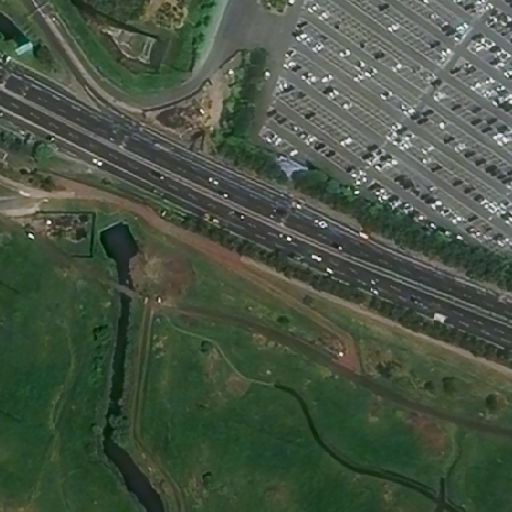
\includegraphics[width=.239\linewidth]{assets/case_rgb.png}&
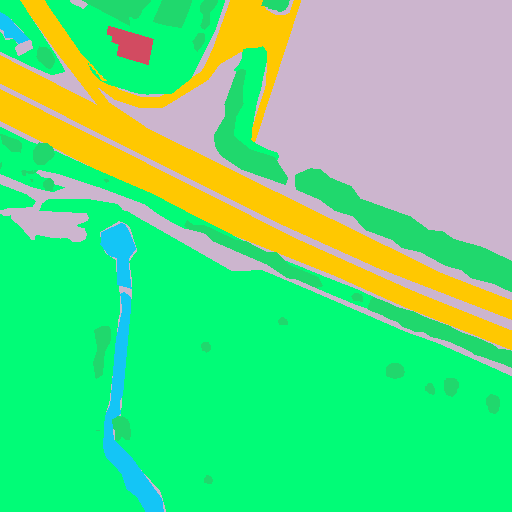
\includegraphics[width=.239\linewidth]{assets/case_gt.png}&
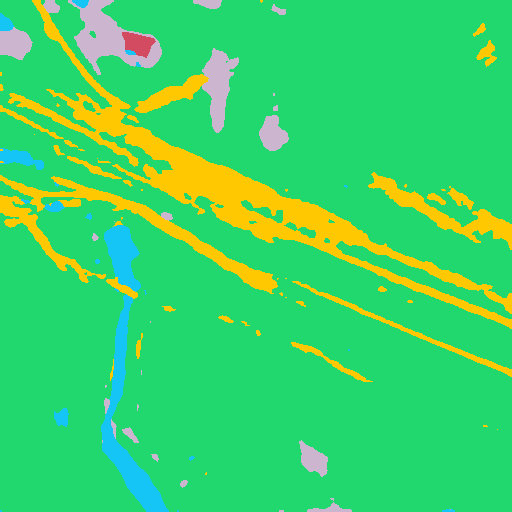
\includegraphics[width=.239\linewidth]{assets/case_official.png}&
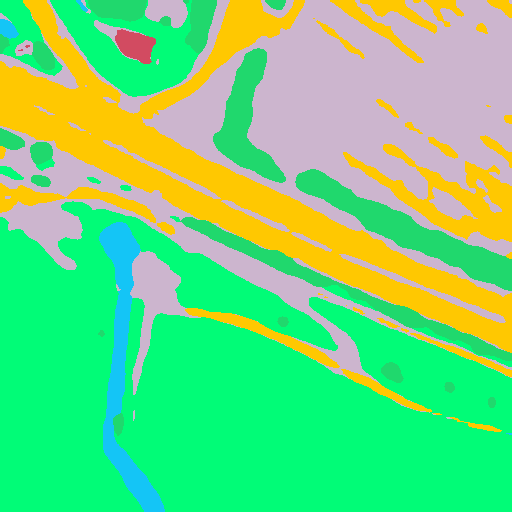
\includegraphics[width=.239\linewidth]{assets/case_finetuned.png}
\end{tabular}
\vspace{3pt}
\par\small
{\footnotesize 八类真值／微调：
\swatch{farmland}{农田}\enspace\swatch{vegetation}{树木}\enspace
\swatch{grass}{草地}\enspace\swatch{water}{水体}\enspace
\swatch{building}{建筑}\enspace\swatch{road}{道路}\enspace
\swatch{sport}{运动场}\enspace\swatch{bare}{裸地}\par
原模型五类：\swatch{building}{建筑}\quad\swatch{road}{道路}\quad
\swatch{bare}{无植被}\quad\swatch{vegetation}{植被}\quad\swatch{water}{水体}}
\caption{测试切片 \texttt{673\_x0512\_y0000}，真值与微调预测保留八类，原模型保留五类。
本图真值出现六类，无农田、运动场。仅在计算共同五类指标时合并类别，mIoU 为
\textbf{40.85\%}$\rightarrow$\textbf{72.65\%}；微调模型本图的八类像素准确率为 83.33\%。}
\end{figure}
\vspace{-5pt}
原模型将右上停车区大面积分为植被；微调后，裸地区域、主干道路与水渠更接近八类真值。
此图按八类逐图 mIoU 约第 95 百分位选取，仅作成功示例；总体效果以上表全测试集结果为准。

\newpage
\section{数据预处理流程}
\begin{figure}[htbp]
\centering
\begin{tikzpicture}[node distance=7mm and 4mm]
\node[block] (d1) {IRSAMap V2 原始数据\\5,869 张 RGB 原图\\及官方合成标签};
\node[block,right=of d1] (d2) {保留官方数据划分\\训练 4,617／验证 340\\测试 912 张原图};
\node[block,right=of d2] (d3) {按 rvwsb 标签映射八类\\水体编码合并\\ID 0 为农田};
\node[block,right=of d3] (d4) {图像与标签同步裁切\\每张 $1024\times1024$\\切成四张 $512\times512$};
\node[block,below=of d4] (d5) {提取共享边界与孔洞\\保留建筑实例分界\\简化并核验几何一致性};
\node[block,left=of d5] (d6) {由顶点生成高斯热图\\标准差 $\sigma=3$ 像素\\三通道归一化};
\node[block,left=of d6] (d7) {D4 增强＋冻结 VAE\\kl-f4，缩放 0.086164\\潜变量 $3\times128\times128$};
\node[block,left=of d7] (d8) {全量验收后供训练使用\\RGB＋八类掩码\\＋对齐的顶点潜变量};
\foreach \a/\b in {d1/d2,d2/d3,d3/d4,d4/d5,d5/d6,d6/d7,d7/d8}
  \draw[flow] (\a) -- (\b);
\end{tikzpicture}
\caption{数据预处理管线。全程由机械程序执行，语义标签以官方合成标签为准。}
\end{figure}
\vspace{-4pt}
最终得到训练 18,468、验证 1,360、测试 3,648 张切片。
训练预计算八种 D4 版本，验证和测试仅保留原方向，共 152,752 个潜变量文件。
验收确认语义掩码与官方映射标签逐像素一致、原图 ID 跨划分无重叠。
八类为农田、树木、草地、水体、建筑、道路区域、运动场和裸地。

\section{模型微调流程}
\begin{figure}[htbp]
\centering
\begin{tikzpicture}[node distance=7mm and 4mm]
\node[block] (t1) {官方 ACPV-Net 权重\\五类语义＋顶点扩散\\VMamba-S＋UPerNet};
\node[block,right=of t1] (t2) {适配八类输出\\重建主、辅助分类层\\其余兼容权重复用};
\node[block,right=of t2] (t3) {先做 300 步小试\\验证前向、反向\\检查点保存与恢复};
\node[block,right=of t3] (t4) {正式重新初始化\\冻结预训练模块\\仅训新分类层 1,000 步};
\node[block,below=of t4] (t5) {联合微调 30,000 步\\更新骨干、语义与扩散\\VAE 保持冻结};
\node[block,left=of t5] (t6) {联合阶段每 2,000 步\\验证全部 1,360 张切片\\计算八类 mIoU};
\node[block,left=of t6] (t7) {按验证 mIoU 选模型\\最优全局步数 25,000\\验证 mIoU 55.39\%};
\node[block,left=of t7] (t8) {固定最佳模型做测试\\3,648 张测试切片\\八类评估与共同五类对照};
\foreach \a/\b in {t1/t2,t2/t3,t3/t4,t4/t5,t5/t6,t6/t7,t7/t8}
  \draw[flow] (\a) -- (\b);
\end{tikzpicture}
\caption{微调与模型选择管线。正式训练从官方权重重新开始，测试集不参与模型选择。}
\end{figure}
\vspace{-4pt}
\textbf{主要设置：}AdamW、有效批量 8、BF16、seed 42；
联合阶段骨干、语义和扩散学习率分别为 $3\times10^{-6}$、$3\times10^{-5}$、$10^{-5}$，
采用预热与余弦衰减。损失为主分支加权交叉熵、0.4 倍辅助交叉熵和 10 倍扩散噪声 L1。
正式训练共 31,000 次更新，使用单张 GPU，耗时约 3 小时 50 分钟。

\vspace{5pt}
{\footnotesize
实验依据：\texttt{official\_vs\_finetuned\_common5.json}、
\texttt{irsamap8\_final\_test\_report.json} 与本轮训练配置。
\href{https://wandb.ai/rykflashv17-tsinghua/acpv-net-irsamap8/runs/l6bw7qcq}{正式训练记录}\quad
\href{https://wandb.ai/rykflashv17-tsinghua/acpv-net-irsamap8/runs/fij4lkv3}{原模型与微调模型对照记录}。}
\end{document}
